\section[Banco de equações]{Banco de equações}
Antes de chegar ao modelo do projeto como está hoje, foi pensado em um modelo anterior. Após algumas reflexões
optou-se seguir por outro caminho considerado mais simples.

\subsection[Como se pensou]{Como se pensou}

No início pensou-se em utilizar um banco de dados relacional para armazenar os metadados e as imagens renderizadas das equações. No Modelo Entidade Relacionamento (MER) modelado inicialmente estavam presentes seis entidades, cada uma com seus atributos. 

\begin{itemize}
	\item EQUAÇÃO\_DIFERENCIAL (linearidade, separável, homogênea, exata e o \underline{id}).
	\item ORDEM (primeira, segunda, terceira, ordem\_superior).
	\item DIFICULDADE (fácil, facilmedio, medio, mediodificil e difícil).
	\item TIPO (ordinária e parcial).
	\item PERGUNTA (img\_src, largura e comprimento).
	\item RESPOSTA (img\_src, largura e comprimento).
\end{itemize}

Houve a reflexão de criar uma entidade pai IMAGEM e fazer com que PERGUNTA e RESPOSTA herdem suas propriedades. Este modelo apesar de incompleto, seria viável para a solução, mas optou-se por não seguir utilizando um banco de dados e \textit{queries}.

\subsection[Como está hoje]{Como está hoje}

Atualmente é utilizado apenas um arquivo \textit{.json} com o dados brutos e de controle.
O projeto banco de equações está disponível em \url{https://github.com/LeonardoRk/TCC-2} dentro da pasta chamada \textbf{banco}. Este projeto visa preparar e validar informações e imagens de perguntas e respostas das equações diferenciais que serão utilizadas no jogo.

O AprEnDO foi populado com as imagens e os metadados fornecidos pelo Wolfran Alpha através de um script de população. O Wolfran Alpha é um serviço online que tem como uma de suas muitas funcionalidades resolver equações diferenciais e apresentar informações quanto à classificação. Com o intuito de realizar requisições à Application Programming Interface API foi criada uma conta gratuita para liberar acesso a uma chave gratuita (chave usada: 3GGQAT-98EG4KV6VL) que permite 2000 requisições por mês. Para se conectar com o Wolfran Alpha foi realizado o \textit{donwload} de uma biblioteca em javascript que pode ser encontrada em: \url{https://products.wolframalpha.com/api/libraries/javascript/} 

Foi desenvolvido um script alimentado por um arquivo de \textit{seeds} que realiza as requisições para a API do Wolfran Alpha para ler os metadados de cada EDO's e guardar/baixar os dados necessários. Os metadados são no formato \textit{JSON}. Eles fornecem a url para a imagem .gif das equações perguntas e respostas (quando existente), estas são utilizadas no jogo, então é necessário mapeá-las em um arquivo index.js para adicionar na pasta resource do jogo no \textit{react native} para fazer com que a internet não seja um requisito para jogar.
 
A Figura \ref{fig:processopopulacao} explica a atividade executada pelo script de população.
O link apresenta a imagem maior \url{https://raw.githubusercontent.com/wiki/LeonardoRk/TCC-2/image/processos/processo_banco_equacoes.png}.  

\begin{figure}[H]
\caption{Processo de script de população}
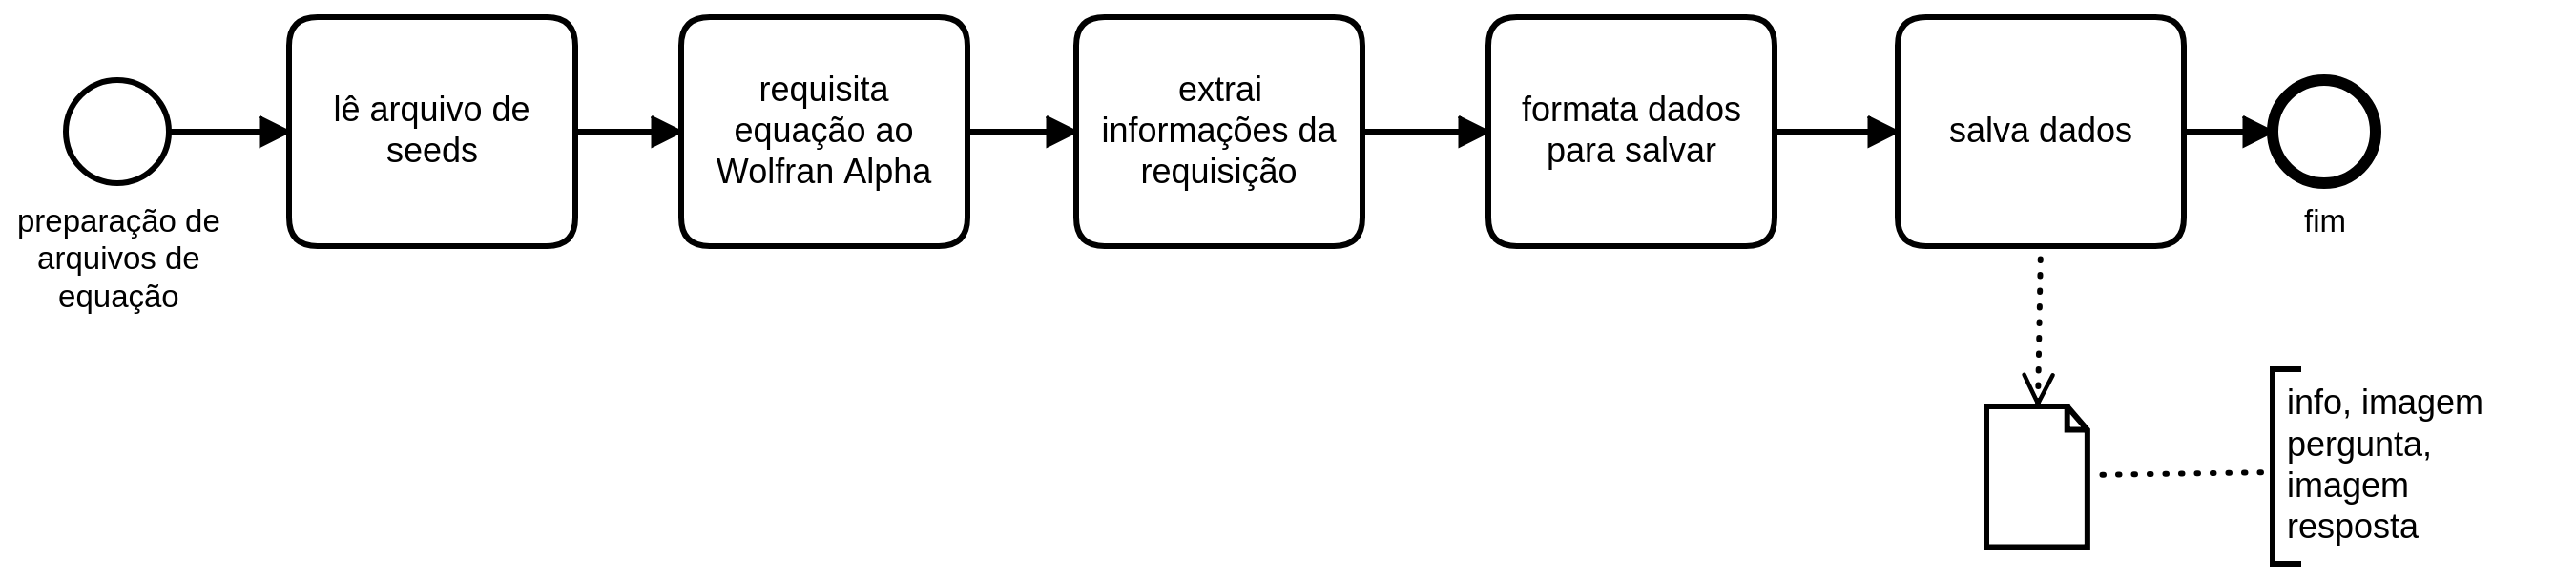
\includegraphics[width=\textwidth,height=\textheight, keepaspectratio]{figuras/processos/processo_banco_equacoes.png}
\label{fig:processopopulacao}
\end{figure}
Na pasta banco existe um arquivo chamado \textbf{seeds.txt} que é o arquivo com as equações diferenciais para alimentar o banco de dados da aplicação aprEnDO. O script \textbf{equações.js} lê o arquivo de seeds equação por equação, faz a requisição para o Wolfran Alpha utilizando os códigos da pasta wolfran\_api e requisita todos os pod disponíveis (pod são os arrays de informação disponibilizados). Após ter os pods são filtradas as informações desejadas e salvas em arquivos de informações localizadas na pasta \textbf{info}. Os pods apresentam as \textit{urls} das imagens de equações de perguntas e respostas, quando existe resposta. Equações sem solução só podem ser utilizadas no primeiro módulo do jogo, o de classificação e não são incluídas no módulo de resolução. As imagens de perguntas baixadas são salvas na pasta \textbf{pergunta} e as imagens de respostas salvas na pasta \textbf{resposta}.

Com todas as informações desejadas de cada equação é possível utilizar o arquivo \textbf{estatisticas.js} que lê todos os arquivos de informação para contabilizar as informações da quantidade de equações diferenciais, quais tem resposta e quais não, quais são homogêneas, exatas, separáveis, linear, não linear, ordem1, ordem2, ordem3, ordem de 4 para cima são consideradas ordem superior, além de fazer a contagem total,também são indicados o número da equação. Essas informações são escritas num arquivo de controle para que possa ser lido pelo aplicativo aprEnDO e fazer a seleção das equações correta para renderizar, a depender do nível que a pessoa está jogando. O nome do arquivo de controle é \textbf{DADOS\_GERAIS.json}.
